\documentclass{article}

%\usepackage[left=2.5cm,right=2.5cm,top=1.5cm,bottom=1.5cm]{geometry}
\usepackage{anysize}
\usepackage{graphicx}
\usepackage{parskip}
\usepackage{amsmath, amsthm, amssymb, amsfonts}

\usepackage{times}

\usepackage[utf8]{inputenc} % this is needed for umlauts
\usepackage[german]{babel} % this is needed for umlauts
\usepackage[T1]{fontenc}    % this is needed for correct output of umlauts in pdf

\usepackage[font=small,labelfont=bf]{caption}

\newcommand{\piMIN}{\pi_\text{MIN}}
\newcommand{\piMAX}{\pi_\text{MAX}}
\newcommand{\pimin}{\pi_\text{min}}
\newcommand{\pimax}{\pi_\text{max}}
\newcommand{\phiMIN}{\varphi_\text{MIN}}
\newcommand{\phiMAX}{\varphi_\text{MAX}}
\newcommand{\phimin}{\varphi_\text{min}}
\newcommand{\phimax}{\varphi_\text{max}}
\newcommand{\LMAX}{L_\text{MAX}}
\newcommand{\LMIN}{L_\text{MIN}}
\newcommand{\Lmax}{L_\text{max}}
\newcommand{\pin}{p_\text{in}}

\begin{document}

\section*{Verdichtermodellierung}

Verdichter sind von allen modellierten Elementen die kompliziertesten. Dies liegt daran, dass zum einen die Verdichtung von Gas gewissen Regeln unterliegt und zum anderen die für die Verdichtung nötige Antriebsenergie auch Beschränkungen hat. 

Normalerweise begreift man einen Verdichter als eine Maschineneinheit aus Antrieb und dem eigentlichen Erdgasverdichter. Beide Aggregate haben ein sogenanntes Kennfeld, das ihren jeweils erlaubten Betriebszustand beschreibt. In unserem Modell vereinfachen wir die Sache sehr: Die relevanten Größen des Antriebs werden mit den Größen des eigentlichen Verdichters in ein gemeinsames Diagramm aufgenommen.

Ein solches zweidimensionales Diagramm wird {\em Kennfeld} genannt. Es beschreibt den zulässigen Bereich, in dem der Verdichter sich befinden muss, wenn er Gas verdichtet. Zulässig ist zusätzlich natürlich immer der Fall, dass der Verdichter inaktiv ist, also gar nicht von Gas durchflossen wird.

Im weiteren Verlauf dieses Artikels wird die Bezeichnung  {\em Kennfeld} mal für das x-y-Diagramm und mal für den in diesem Diagramm erlaubten Bereich des Verdichterzustands verwendet. Aus dem Kontext sollte aber ersichtlich sein, wie die Bezeichnung jeweils verwendet wird.


\section{Aufbau des Kennfelds}
Unser Kennfeld (siehe Abb. \ref{fig:kf}) ist ein x-y-Diagramm, das den erlaubten Bereich (zuweilen eben auch Kennfeld genannt) des Verdichterzustands definiert. Auf der x-Achse steht der Betriebsvolumenfluss $\varphi$ durch den Verdichter, auf der y-Achse das Druckverhältnis $\pi:=\frac{p_{\text{out}}}{p_{\text{in}}}$ aus Ausgangs- und Eingangsdruck.

%\begin{equation}
%\pi:=\frac{p_{\text{out}}}{p_{\text{in}}}
%\label{eq:pi}
%\end{equation}


\begin{figure}[!ht]
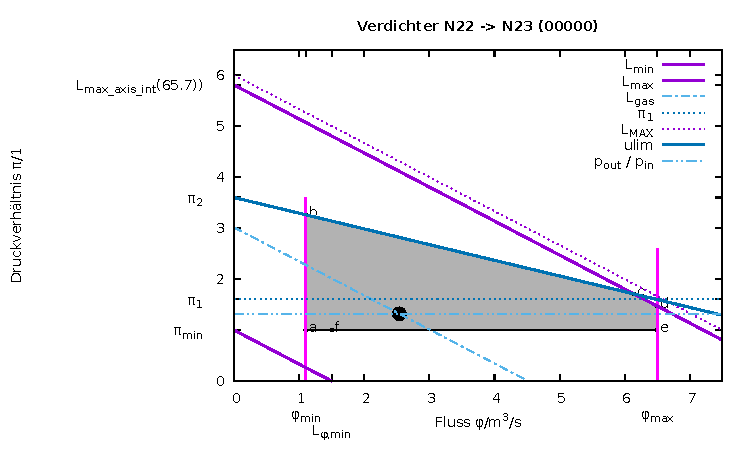
\includegraphics[width=0.9\textwidth]{Example_Compressor_Wheel_Map.pdf}
\caption{Für unsere Zwecke vereinfachtes Verdichterkennfeld, das neben den Kenndaten für den eigentlichen Verdichter auch die Antriebsleistung enthält.}
\label{fig:kf}
\end{figure}



Auf der x-Achse sind zwei Konstanten definiert, die das Kennfeld links und rechts begrenzen, 
$\varphi_\text{min}$ ist der minimal zulässige Fluss und $\phimax$ der maximal zulässige. Auf der y-Achse definiert $\pimin$ das minimal zulässige Druckverhältnis, es hat üblicherweise den Wert 1.

\section{Antriebsleistungen}

Für einen Verdichter sind durch seinen Antrieb drei Leistungen definiert, die in unserem vereinfachten Modell durch parallele Geraden modelliert werden:

\begin{enumerate}

\item Minimalleistung; Gerade durch $(0,\piMIN)$ und $(\phiMIN,0)$
$$L_\text{MIN}: \begin{pmatrix} 0 \\ \piMIN \end{pmatrix} + \lambda \begin{pmatrix} \phiMIN - 0 \\ 0 - \piMIN \end{pmatrix},\text{ bzw. } \LMIN(\varphi)=-\frac{\piMIN}{\phiMIN}\varphi+\piMIN$$


\item Absolute Maximalleistung; Parallele zu $L_\text{MIN}$ durch $(0,\pi_{\text{MAX}})$
$$\LMAX: \begin{pmatrix} 0 \\ \pi_{\text{MAX}} \end{pmatrix} + \lambda \begin{pmatrix} \phiMIN - 0 \\ 0 - \piMIN \end{pmatrix},\text{ bzw. } L_{\text{MAX}}(\varphi)=-\frac{\piMIN}{\phiMIN}\varphi+\piMAX$$

\item Aktuelle Maximalleistung; Parallele zu $L_\text{MIN}$ durch $(0,\pimax)$
$$\Lmax(\pimax): \begin{pmatrix} 0 \\ \pimax \end{pmatrix} + \lambda \begin{pmatrix} \phiMIN - 0 \\ 0 - \piMIN \end{pmatrix},\text{ bzw. } \Lmax(\varphi)=-\frac{\piMIN}{\phiMIN}\varphi+\pimax$$


\end{enumerate}

Die Minimalleistung gibt an, welche Leistung nicht unterschritten werden darf, wenn der Verdichter aktiv ist. Zusätzlich ist immer eine Leistung von Null erlaubt, die dann gilt, wenn der Verdichter inaktiv ist.

Die aktuelle Maximalleistung hängt durch eine Funktion $\pimax$ vom aktuellen Eingangsdruck $p_\text{in}$ ab.
$$\pimax: p_\text{in} \longmapsto \piMAX \left( (\eta - 1) \frac{\pin - \pin^{\text{min}}}{\pin^{\text{max}} - \pin^{\text{min}}} + 1 \right)$$
Dabei wird der Parameter $\eta$  dazu genutzt, die Abhängigkeit der aktuellen Maximalleistung vom Eingangsdruck zu modellieren. Für $\eta=1$ liegt keine Abhängigkeit vor und es gilt $\LMAX=\Lmax $.
 
\section{Kennfeldgrenzen}

Die Gerade U durch die Punkte $(0, \pi_2)$ und $(\phimax, \pi_1)$ dient dazu, das Kennfeld nach oben zu begrenzen.
Dabei beschreibt $\pi_2$  gewissermaßen das maximale Druckverhältnis bei Nullfluss und $\pi_1$ das minimale Druckverhältnis bei maximalem Fluss.
$$U: \begin{pmatrix} 0 \\ \pi_2 \end{pmatrix} + \lambda \begin{pmatrix} \phimax - 0 \\ \pi_1 - \pi_2 \end{pmatrix},\text{ bzw. } U(\varphi)=\frac{(\pi_1-\pi_2)}{\phimax}\varphi+\pi_2$$


Das Kennfeld ist ein Sechseck mit den Eckpunkten a bis f, die folgendermaßen definiert sind:
\begin{description}

\item[a]  Punkt $(\varphi_\text{min},L_\text{MIN}(\varphi_\text{min}))$
\item[b]  Punkt $(\varphi_\text{min}, U(\phimin))$
\item [c] Schnittpunkt der beiden Geraden $U$ und $\Lmax$
\item [d] Punkt $(\phimax, \Lmax(\phimax))$
\item [e] Punkt ($\phimax, \pimin)$  
\item [f] Punkt $(\LMIN^{-1}(\pimin), \pimin)$ 

\end{description}


\section{ Bestimmung des Arbeitspunktes und des Flusses}

Arbeitspunkt eines Verdichters wird derjenige Punkt im Kennfeld genannt, der den aktuellen Fluss durch den Verdichter und das aktuelle Druckverhältnis abbildet. Der Arbeitspunkt wird vom Simulator festgelegt aufgrund der Aktivitäten des Dispatcher-Agenten.

Der Dispatcher-Agent darf sich wünschen, ob der Verdichter aktiv ist
oder nicht. Dem Wunsch auf Inaktivität wird immer entsprochen, dem auf
Aktivität nicht. Dies liegt daran, dass der Arbeitspunkt $A$ eines aktiven Verdichters immer im Kennfeld $K$
liegen muss und immer auf der durch $\pi$ spezifizierten Geraden $\Pi$. Falls diese beiden Mengen disjunkt sind, so ist der Verdichter zwingend inaktiv, auch wenn der Dispatcher-Agent sich einen aktiven Verdichter wünscht.

Der Wunsch auf Aktivität muss immer mit einer Wunschleistung $W$ verbunden
sein. $W$ liegt zwischen 0\% und 100\% und wird vom Simulator linear auf eine
Leistung $L$ umgerechnet, die zwischen $\LMIN$ und $\Lmax$ liegt.

Es gibt immer einen Schnittpunkt $S$ von $L$ und $\Pi$. Liegt $S$ in $K$, so ist $A = S$. Liegt $S$ nicht in $K$, so ist $S$ der nächstgelegene Randpunkt von $K$, der auf
$\Pi$ liegt. Per Konstruktion muss es einen solchen Punkt geben:

\begin{enumerate}
\item Bilde $D$ als Schnittstrecke von $\Pi$ und $K$.
\item Bilde $S$ als Schnittpunkt von $\Pi$ und $L$.
\item Dann ist $A$ der $S$ nächstgelegene Punkt aus $D$.

\end{enumerate}

Der Simulator nutzt den ermittelten Arbeitspunkt, um seine eigentlich Aufgabe zu erfüllen: aus einer Wunschleistung des Dispatcher-Agenten den Fluss über den Verdichter zu bestimmen. 


\end{document}
